% -------------------------------------------------------
%  ___ ___  _ __ ___  _ __   __ _ _ __ ___ 
% / __/ _ \| '_ ` _ \| '_ \ / _` | '__/ _ \
%| (_| (_) | | | | | | |_) | (_| | | |  __/
% \___\___/|_| |_| |_| .__/ \__,_|_|  \___|
%                    |_|                   
% -------------------------------------------------------
\chapter{Models Comparison}

As mentioned earlier \ref{sec:digital_twin}, the simulation model can be used in several
situations.  Models of the normal condition can simulate system output to a
given input in normal operating conditions. This type of model can be used
to provide, for example, residual estimation. Compare normal condition
model with measured signals from sensors decision algorithm can evaluate
possible faults. 

Suppose the model can simulate the system in different conditions. In that
case, it gives an option to implement  "What-If" simulations and prevent
fault situations that are not captured in the measured dataset.

No best solution would apply in all situations, but for a specific example
of the double-acting pneumatic actuator with the measured dataset, the more
efficient model can be evaluated. Table \ref{tab:models_compare} represents the comparison
simulation models in 4 categories, simulation speed, accuracy concerning
the actual model, the difficulty of deploying the model, the behavior under
normal conditions and the possibility of simulating abnormal "What-If"
situations.

The speed of the simulation or calculation complexity performs a more
prominent role in the model's design, especially during the estimation of
the parameters, where the simulations are performed hundreds of times in a
row.

\begin{table}[h]
    \centering
    \begin{tabular}{|c|c|c|c|c|}
\hline
\textbf{model} &\textbf{speed} &\textbf{accuracy} &\textbf{normal cond.} &\textbf{abnormal} \\
\hline
FPM            & fast          & normal           & yes                  & yes \\
Simscape       & low           & normal           & yes                  & yes \\
HW model       & fast          & very low         & -                    & - \\
NARX           & fast          & high             & yes                  & - \\
\hline
    \end{tabular}
    \caption{Models developed by different approach comparison}
    \label{tab:models_compare}
\end{table}
    
\todo[inline]{Text}

%\section{First Principle Model}
%This model \ref{fig:model_equations} was developed with respect to equations
%represented before.
%
%\begin{figure}[h!]
%    \centering
%    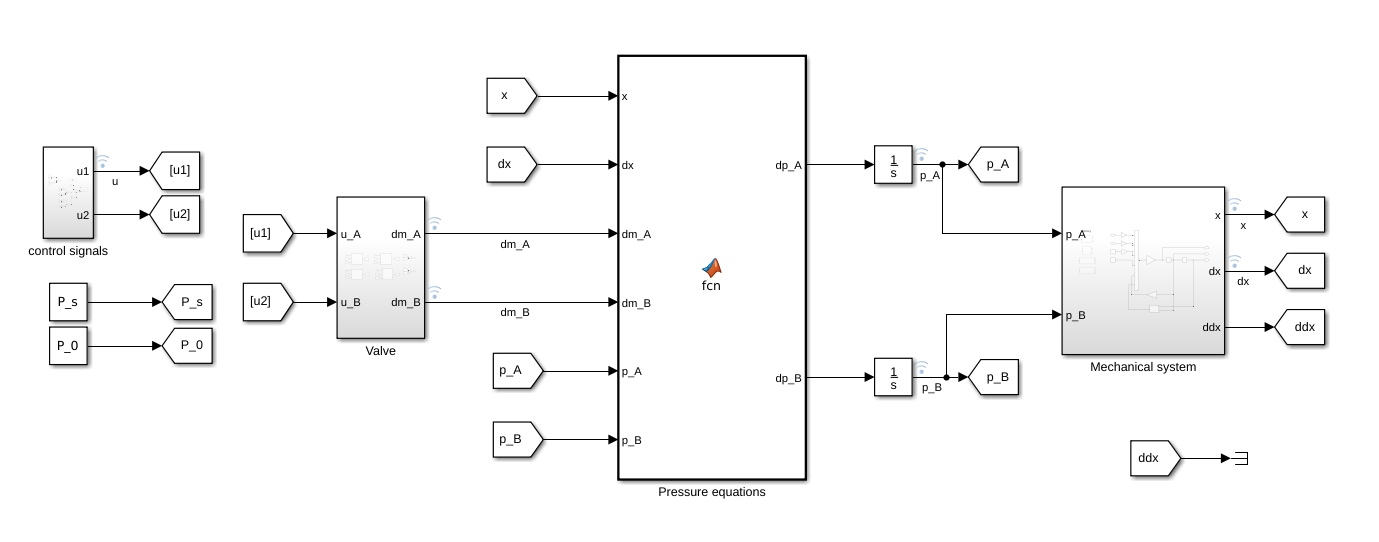
\includegraphics[width=1\textwidth]{equations.png}
%    \caption{Simulink model based on equations}
%    \label{fig:model_equations}
%\end{figure}
%
%\section{Alternative Modeling Techniques (3 pages)}
%Generally with dataset of input-output signals approximation model can be
%fit. Using System Identification Toolbox and modeled as Black-Box or
%Gray-Box models. This section attempted to fit some models using data from
%SimScape and Equation model presented before.
%
%Fit approximation model make sense only if we know what to fit. Using
%signal process techniques and identify dominant signals that providing best
%classification features we will train models with respect to this signals.
%
%\subsection{Physical Model (SimScape)}
%Working, very slow. Equations are faster for estimation parameters.
%Model \ref{fig:model_simscape} was developed using SimScape toolbox.
%
%\begin{figure}[h!]
%    \centering
%    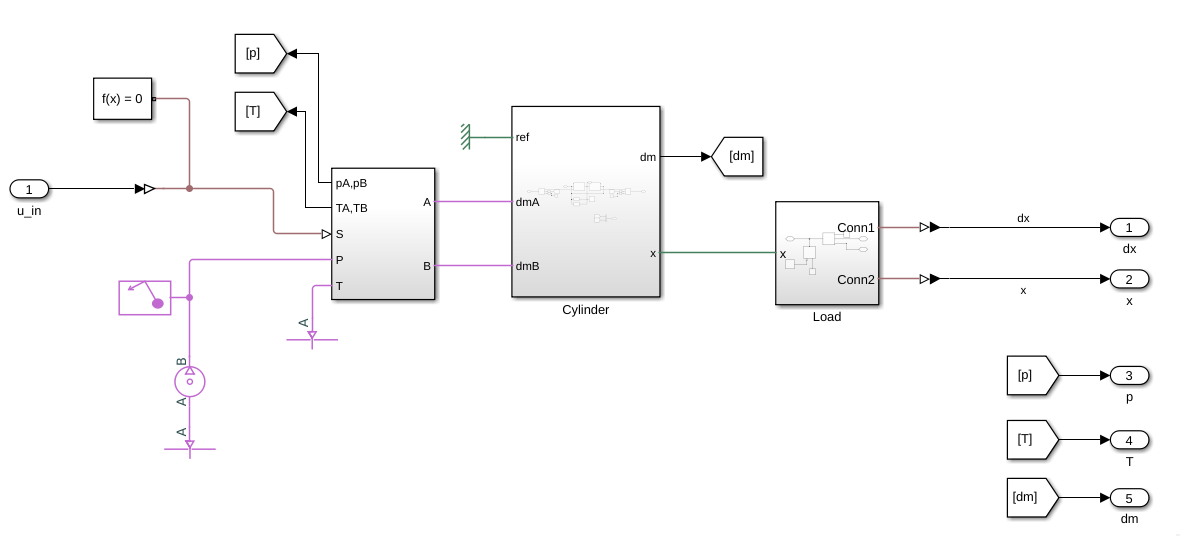
\includegraphics[width=1\textwidth]{simscape.png}
%    \caption{Simulink model using SimScape Toolbox}
%    \label{fig:model_simscape}
%\end{figure}
%
%\subsection{State-space/ARX Models}
%Not working, Nonlinearities.
%
%
%\subsection{Hammerstein-Wiener Model}
%Working only for Position.
%
%\subsection{Nonparametric model (ANN)}
%
%Working. Can be used as "Normal operation" model.
%
%
%
%\section{Comparison}
%Following figure \ref{fig:compare_of_models} represent comparison of 2 models
%(Simscape and based on equations) using same parameters for simulation:
%There is slight difference between models causing Valve dynamics
%simplifications in model based on equations.
%
%\begin{figure}[h!]
%    \centering
%    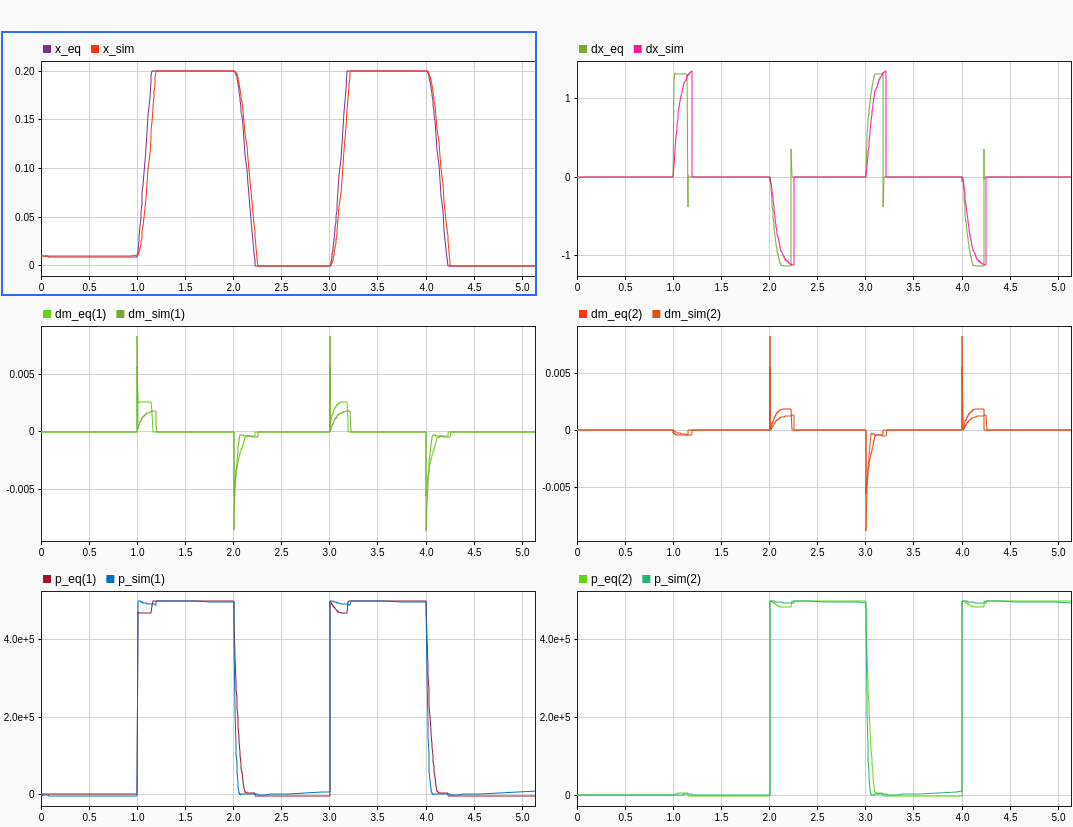
\includegraphics[width=0.8\textwidth]{models_comparation.png}
%    \caption{Comparison of simscape and model based on equations}
%    \label{fig:compare_of_models}
%\end{figure}
%
%
